% ************************************************************************
%\documentclass[12pt,oneside,letterpaper]{article}
% ************************************************************************
%\usepackage[small,bf]{caption}
%\renewcommand{\thefigure}{S\arabic{figure}}
%\usepackage{cite}
%\usepackage{times}
%\usepackage{helvet}
%\usepackage{epsf}
%\usepackage{graphicx}
%\usepackage{graphbox}
%\usepackage{amsmath}
%\usepackage[mathscr]{euscript}
%\usepackage{algorithm}
%\usepackage{algpseudocode}
%\usepackage{multirow}
% ************************************************************************
%\columnsep        0.0in
%\evensidemargin   0.0in
%\footskip         0.2in
%\headheight       0.3in
%\headsep          0.3in
%\hoffset          0.0in
%\marginparpush    0.0in
%\marginparsep     0.0in
%\marginparwidth   0.0in
%\oddsidemargin    0.0in
%\paperheight     11.0in
%\paperwidth       8.5in
%\tabcolsep        0.0in
%\textheight       8.8in
%\textwidth        6.5in
%\topmargin        0.0in
%\voffset         -0.25in
%\parindent        0.0em
%\parskip          0.0em
% ************************************************************************
%\usepackage{fancyhdr}
%\pagestyle{fancyplain}
%\renewcommand{\sectionmark}[1]{}{}
%\renewcommand{\subsectionmark}[1]{}
%\lhead[\fancyplain{}{}]{\fancyplain{}{}}
%\chead[\fancyplain{}{}]{\fancyplain{}{}}
%\rhead[\fancyplain{}{}]{\fancyplain{}{}}
%\lfoot[\fancyplain{}{}]{\fancyplain{}{}}
%\cfoot[\fancyplain{}{}]{\fancyplain{}{\thepage}}
%\rfoot[\fancyplain{}{}]{\fancyplain{}{}}
%\renewcommand{\headrulewidth}{0pt}
%\renewcommand{\footrulewidth}{0pt}

% ************************************************************************
%\begin{document}
% ************************************************************************
%\thispagestyle{empty}
%
%\begin{center}
%
%\vspace*{10\baselineskip}
%
%{\huge\sffamily Automated neuron tracing using\\[0.5em] probability hypothesis density filtering}
%
%\vspace{2\baselineskip}
%
%{\large Miroslav Radojevi{\'c} and Erik Meijering}
%
%\vspace{2\baselineskip}
%
%{\large\bfseries Supplementary Information}
%
%\end{center}
\clearpage
\begin{figure}[!t]
\centering
\begin{tabular}{c@{\hspace{1em}}c@{\hspace{1em}}c}
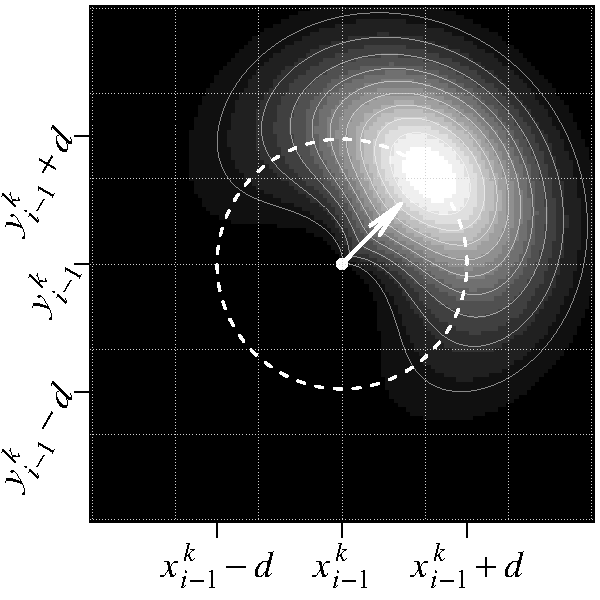
\includegraphics[height=0.3\columnwidth]{./fig/pi} &
\includegraphics[height=0.3\columnwidth]{./fig/beta} &
\includegraphics[height=0.3\columnwidth]{./fig/h} \\
(A) $\pi_{k|k-1}(\mathrm{x}|\mathrm{x'})$ & (B) $\beta_{k|k-1}(\mathrm{x}|\mathrm{x'})$ & (C) $h(\mathrm{p}|\mathrm{x'})$ \\
\end{tabular}  		
\caption{Transition densities (2D examples) for persistent (A) and spawned (B) objects with $z=0$, $\mathrm{x'}=\left[ 0,0,0, \tfrac{1}{\sqrt{2}},\tfrac{1}{\sqrt{2}}, 0 \right] $, $\kappa=2$, and $r_k=3$. (C) Importance sampling used in the observation model without the tubularity component, $\tau(\mathrm{p})=1$, and $\kappa=0.5$. Rainbow color coding is used running from blue (indicating low values) to red (indicating high values).}
\label{fig:transitions}
\end{figure}

% ************************************************************************
\clearpage
\begin{figure}[!t]
\centering
\begin{tabular}{c@{\hspace{2em}}c}
\includegraphics[width=0.4\columnwidth]{./fig/o1} &
\includegraphics[width=0.4\columnwidth]{./fig/o2} \\[-1ex]
(A) $\mathrm{p}_{i}^{n} \sim h(\mathrm{p} | \hat{\mathrm{x}}_{k-1,i})$ &
(B) $\mathrm{p}_{i,j}^n \in \mathscr{C}_j$ \\[3ex]
\includegraphics[width=0.4\columnwidth]{./fig/o3} &
\includegraphics[width=0.4\columnwidth]{./fig/Cz} \\[-1ex]
(C) $\mathrm{z}_{k,j}$ &
(D) $C_k(\mathrm{z}) = e^{-K_c\tau_{\mathrm{z}}}$ 
\end{tabular}
\caption{Formation of the observations (2D example). (A) For each object $i$ from iteration $k-1$, particles $\mathrm{p}_{i}^{n}$ are sampled from the importance sampling function $h$, using the state estimate $\hat{\mathrm{x}}_{k-1,i}$. The solid dot indicates the location of $\hat{\mathrm{x}}_{k-1,i}$ and the contours represent lines of equal particle weight. (B) The particles are processed by mean-shifting resulting in clusters $\mathscr{C}_j$ whose labeled particles are denoted as $\mathrm{p}_{i,j}^{n}$. (C) Each observation $\mathrm{z}_{k,j}$ is obtained from the representative cluster particle $\mathrm{p}_{i,j}^{\hat{n}}$ as described in the main text. Contours represent lines of equal observation likelihood. (D) The clutter intensity function.} 
\label{fig:observation-model}
\end{figure}

% ************************************************************************
\clearpage
\begin{figure}[!t]
\centering
\begin{tabular}{c@{\hspace{1ex}}c@{\hspace{1ex}}c@{\hspace{3ex}}c@{\hspace{1ex}}c@{\hspace{1ex}}c}
(A) &
\includegraphics[align=c,width=0.2\columnwidth]{./fig/101_accno} &% ./fig/opfA/101/acc[no]
\includegraphics[align=c,width=0.2\columnwidth]{./fig/101_accround3} &% ./fig/opfB/101/acc[round]3
(B) &
\includegraphics[align=c,width=0.2\columnwidth]{./fig/109_accno} &% ./fig/opfA/109/acc[no]
\includegraphics[align=c,width=0.2\columnwidth]{./fig/109_accround3} \\% ./fig/opfB/109/acc[round]3
\vspace{-2ex} \\
(C) &
\includegraphics[align=c,width=0.2\columnwidth]{./fig/104_accno} &% ./fig/opfA/104/acc[no]
\includegraphics[align=c,width=0.2\columnwidth]{./fig/104_accround3} &%./fig/opfB/104/acc[round]3
(D) &
\includegraphics[align=c,width=0.2\columnwidth]{./fig/106_accno} &% ./fig/opfA/106/acc[no]
\includegraphics[align=c,width=0.2\columnwidth]{./fig/106_accround3} \\% ./fig/opfB/106/acc[round]3
\vspace{-2ex} \\
(E) &
\includegraphics[align=c,width=0.2\columnwidth]{./fig/301_accno} &% ./fig/sariaA/301/acc[no]
\includegraphics[align=c,width=0.2\columnwidth]{./fig/301_accround} &% ./fig/sariaB/301/acc[round]
(F) &
\includegraphics[align=c,width=0.2\columnwidth]{./fig/302_accno} &% ./fig/sariaA/302/acc[no]
\includegraphics[align=c,width=0.2\columnwidth]{./fig/302_accround} \\% ./fig/sariaB/302/acc[round]
\vspace{-2ex} \\
(G) &
\includegraphics[align=c,width=0.2\columnwidth]{./fig/305_accno} &% ./fig/sariaA/305/acc[no]
\includegraphics[align=c,width=0.2\columnwidth]{./fig/305_accround} &% ./fig/sariaB/305/acc[round]
(H) &
\includegraphics[align=c,width=0.2\columnwidth]{./fig/306_accno} &% ./fig/sariaA/306/acc[no]
\includegraphics[align=c,width=0.2\columnwidth]{./fig/306_accround} \\% ./fig/sariaB/306/acc[round]
\end{tabular}
\caption{Performance as a function of numbers of seeds and rounds for four example cases from the OPF (A-D) and the HCN (E-H) data set. Similar trends were observed for all cases in the respective data sets. Left panel per case: Precision (P), recall (R), and F-score (F) after one round initialized with different numbers of seeds ($N_0$). Right panel per case: The scores after multiple rounds with a fixed number of seeds ($N_0=40$). Fifth-order polynomial curves were fit to the data to show approximate trends.}
\label{fig:opf-saria-tests}
\end{figure}

% ************************************************************************
\clearpage
\begin{figure}[!t]
\centering
\begin{tabular}{c@{\hspace{0.02\columnwidth}}c@{\hspace{0.02\columnwidth}}c}
\includegraphics[width=0.31\columnwidth]{./fig/p_opf} &% ./fig/compare/opf/p
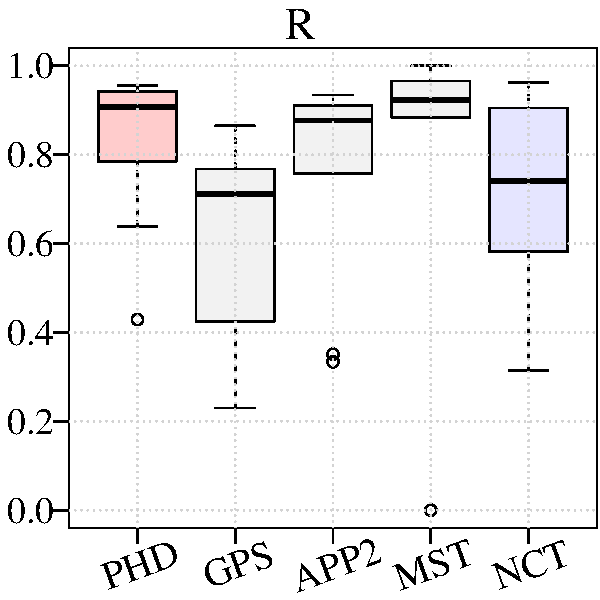
\includegraphics[width=0.31\columnwidth]{./fig/r_opf} &% ./fig/compare/opf/r
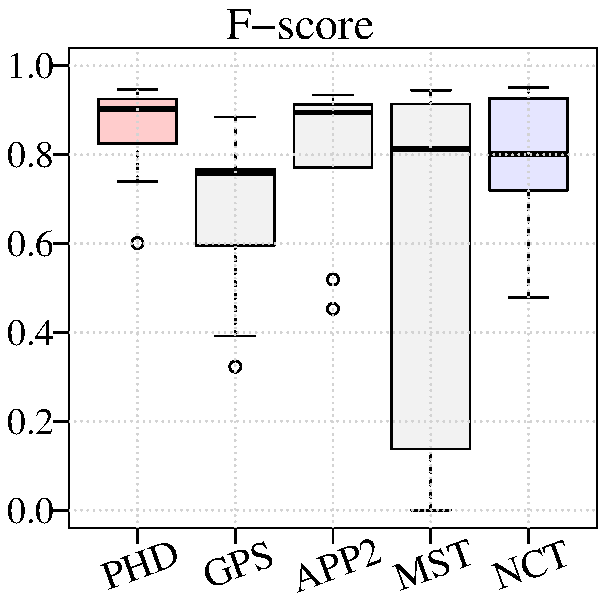
\includegraphics[width=0.31\columnwidth]{./fig/f_opf} \\[1ex]% ./fig/compare/opf/f
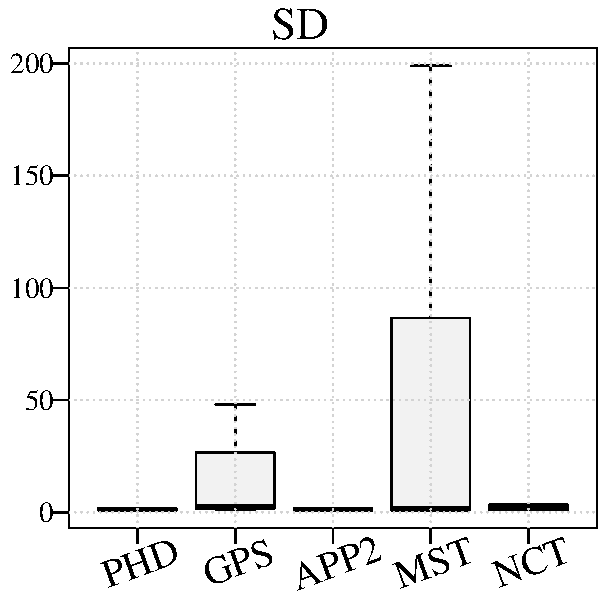
\includegraphics[width=0.31\columnwidth]{./fig/sd_opf} &% ./fig/compare/opf/sd
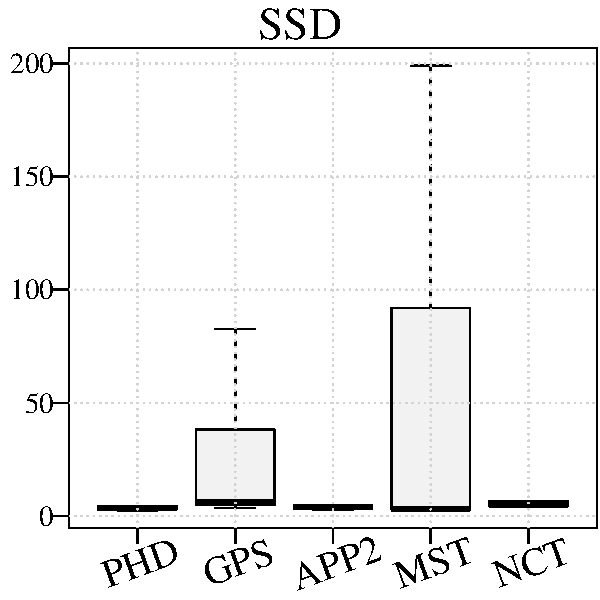
\includegraphics[width=0.31\columnwidth]{./fig/ssd_opf} &% ./fig/compare/opf/ssd
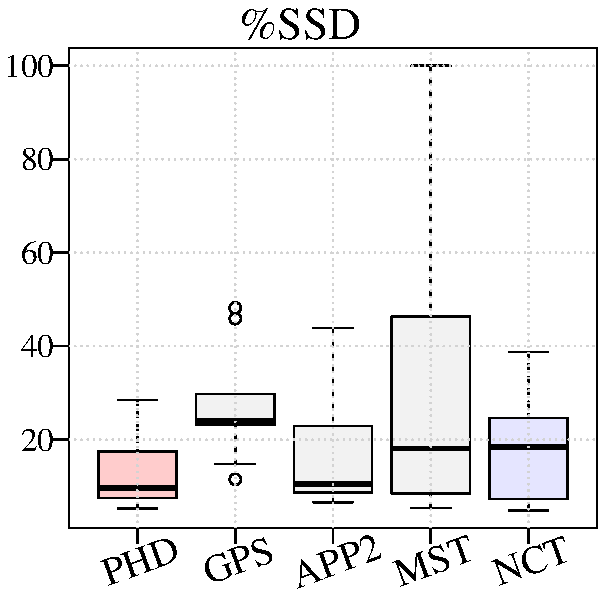
\includegraphics[width=0.31\columnwidth]{./fig/pssd_opf} \\% ./fig/compare/opf/pssd
\end{tabular}
\caption{Performance comparison of our method with several other methods on the OPF data set. For each method and each measure, the plotted box indicates the 25-75 percentile, the horizontal bar indicates the median score, and the whiskers and outliers are drawn using the default settings of R.}
\label{fig:compare-opf}
\end{figure}

% ************************************************************************
\clearpage
\begin{figure}[!t]
\centering
\begin{tabular}{c@{\hspace{0.02\columnwidth}}c@{\hspace{0.02\columnwidth}}c}
\includegraphics[width=0.31\columnwidth]{./fig/p_saria} &% ./fig/compare/saria/p
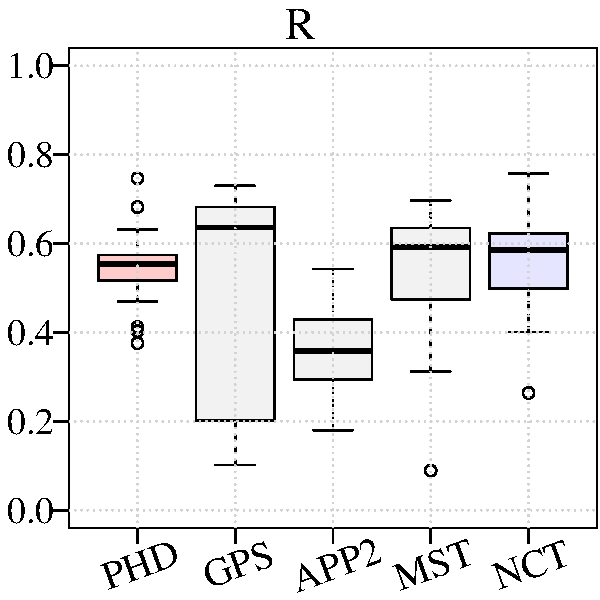
\includegraphics[width=0.31\columnwidth]{./fig/r_saria} &% ./fig/compare/saria/r
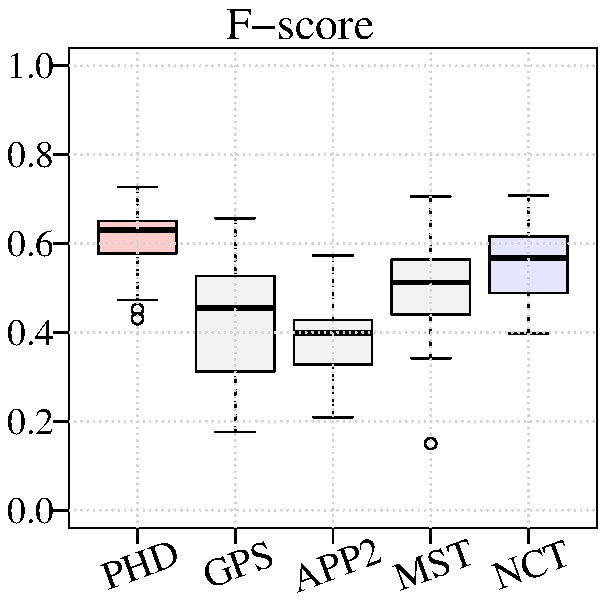
\includegraphics[width=0.31\columnwidth]{./fig/f_saria} \\[1ex]% ./fig/compare/saria/f
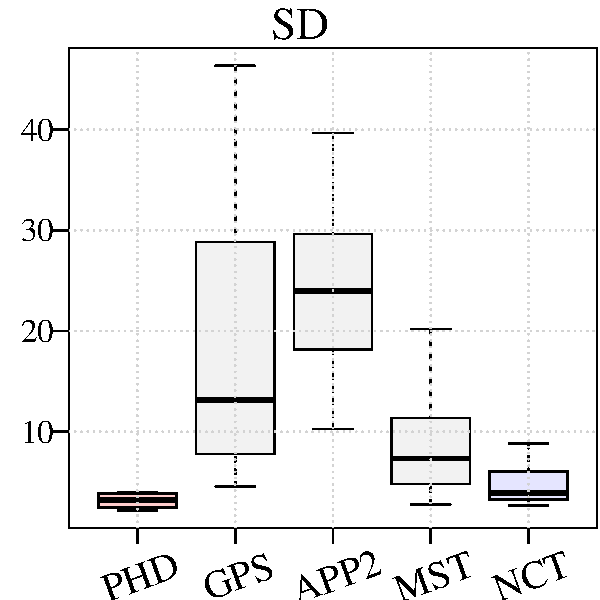
\includegraphics[width=0.31\columnwidth]{./fig/sd_saria} &% ./fig/compare/saria/sd
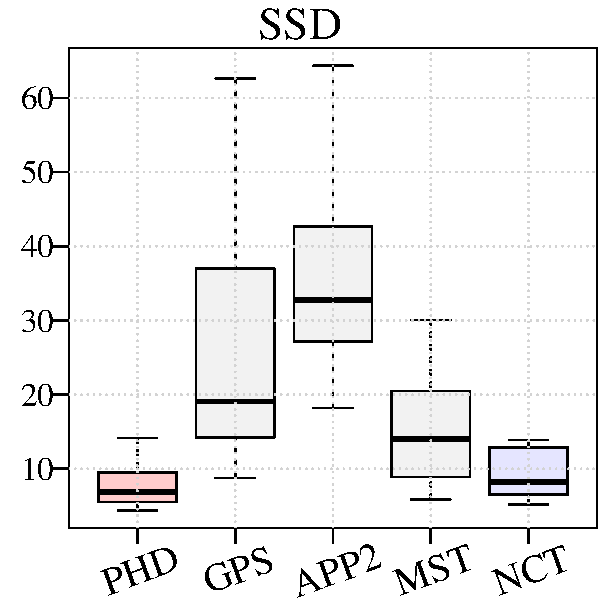
\includegraphics[width=0.31\columnwidth]{./fig/ssd_saria} &% ./fig/compare/saria/ssd
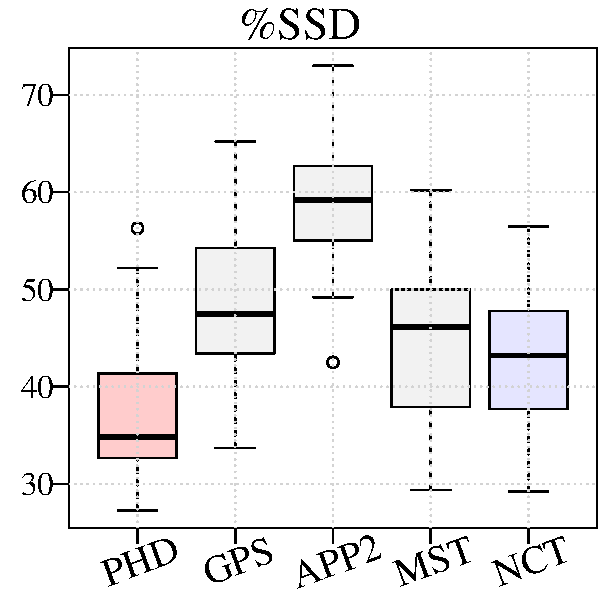
\includegraphics[width=0.31\columnwidth]{./fig/pssd_saria} \\% ./fig/compare/saria/pssd
\end{tabular}
\caption{Performance comparison of our method with several other methods on the HCN data set. For each method and each measure, the plotted box indicates the 25-75 percentile, the horizontal bar indicates the median score, and the whiskers and outliers are drawn using the default settings of R.}
\label{fig:compare-saria}
\end{figure}

% ************************************************************************
\clearpage
\begin{figure}[!t]
\centering
\begin{tabular}{r@{\hspace{0.02\columnwidth}}c@{\hspace{0.02\columnwidth}}c@{\hspace{0.02\columnwidth}}c}
Case: &

\includegraphics[align=c,width=0.15\columnwidth]{./fig/c2.compare/i1_inv} &

\includegraphics[align=c,width=0.15\columnwidth]{./fig/c2.compare/i2_inv} &

\includegraphics[align=c,width=0.15\columnwidth]{./fig/c2.compare/i3_inv}\\
PHD: &
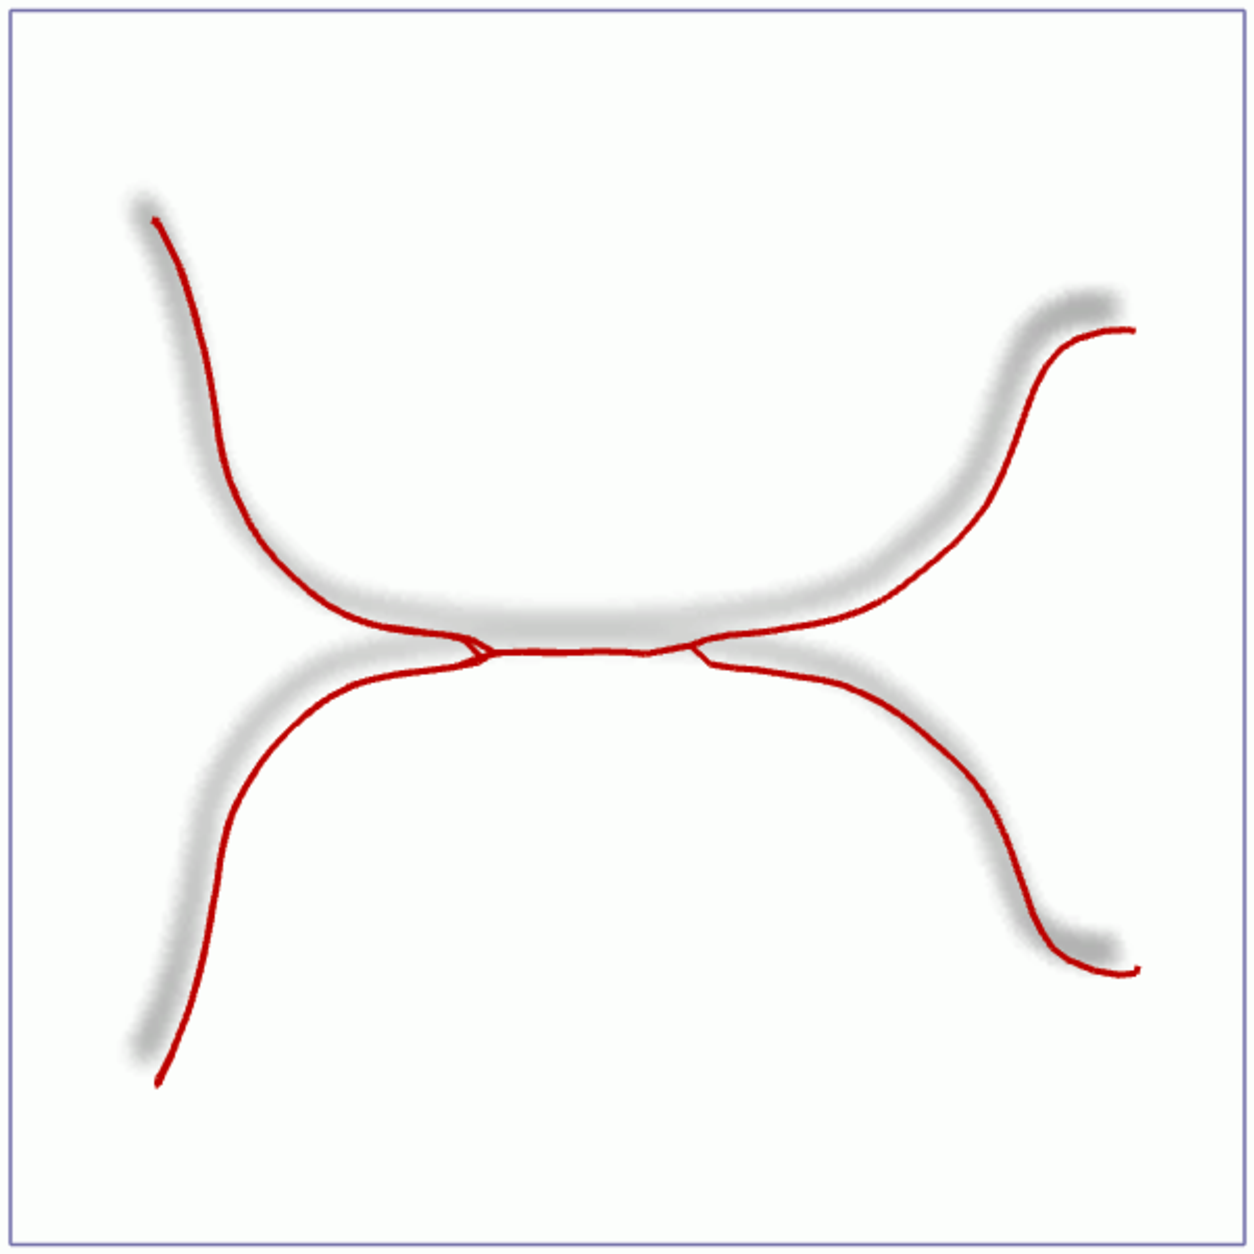
\includegraphics[align=c,width=0.2\columnwidth]{./fig/c2.compare/phd,i1,c0,s0} &
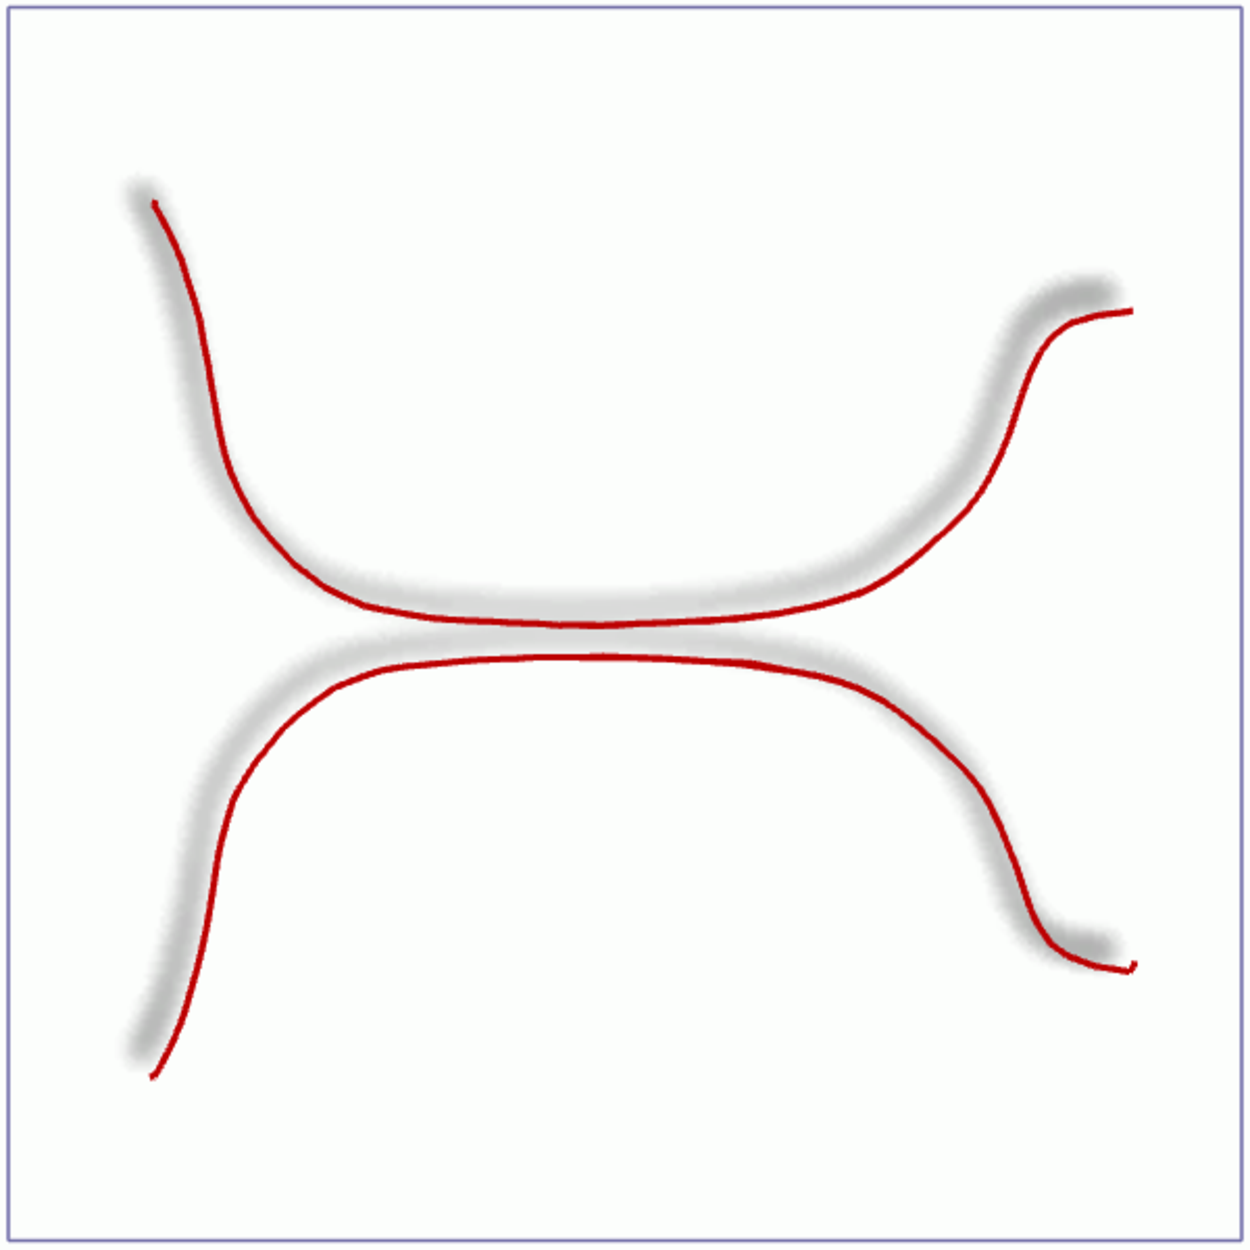
\includegraphics[align=c,width=0.2\columnwidth]{./fig/c2.compare/phd,i2,c0,s0} &
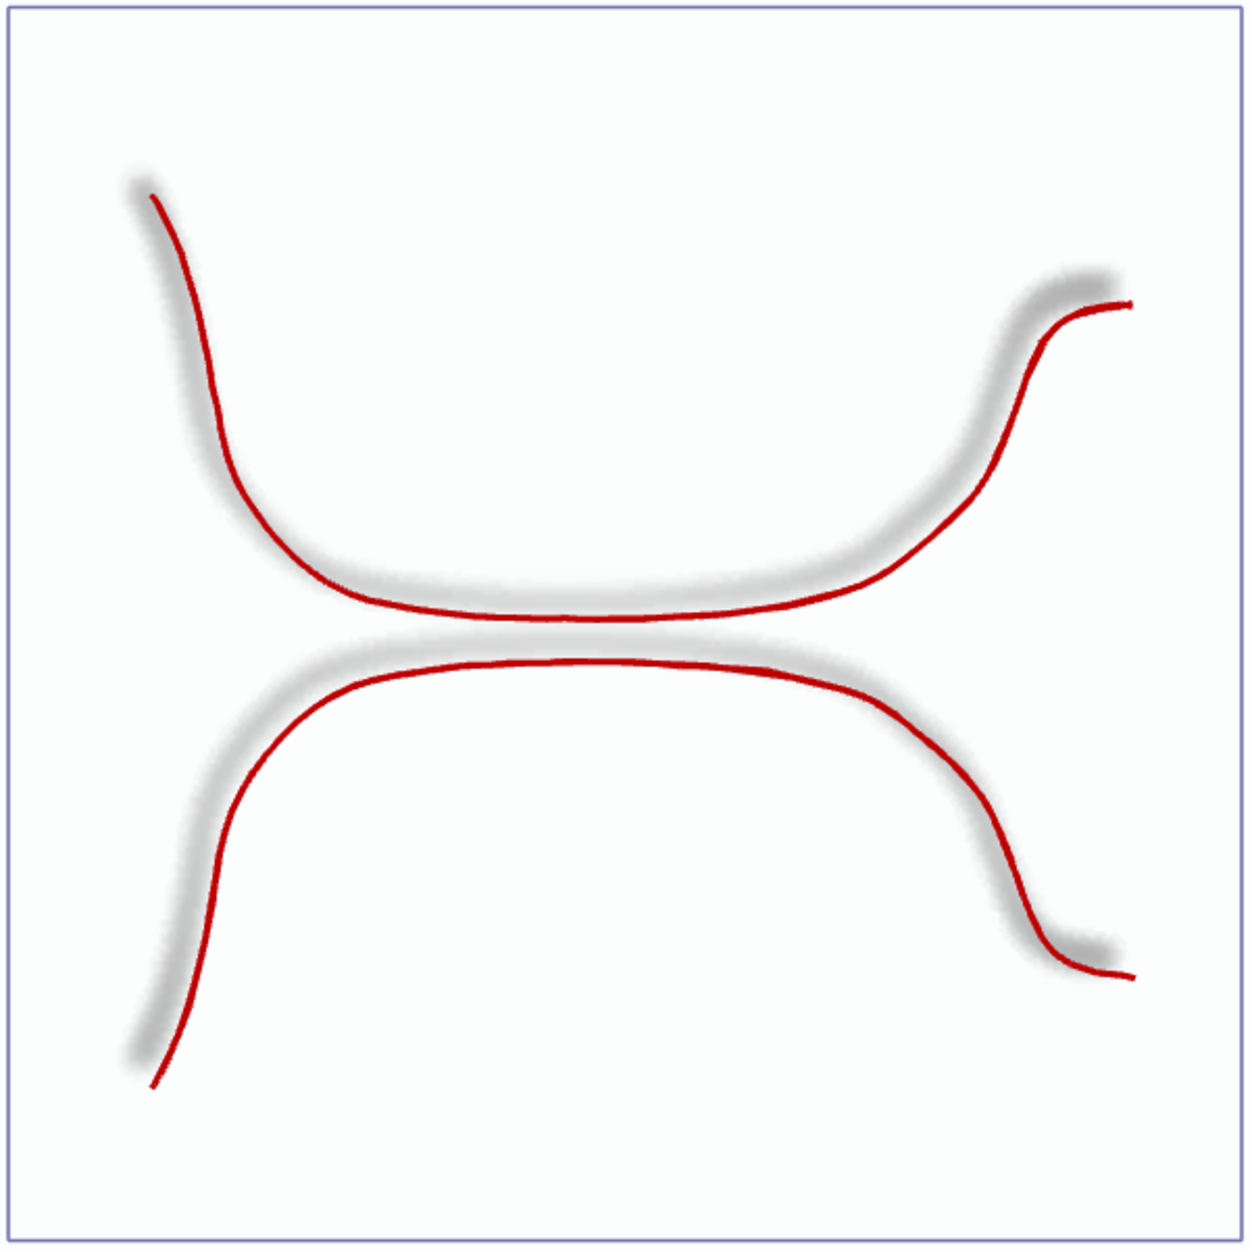
\includegraphics[align=c,width=0.2\columnwidth]{./fig/c2.compare/phd,i3,c0,s0} \\
GPS: &
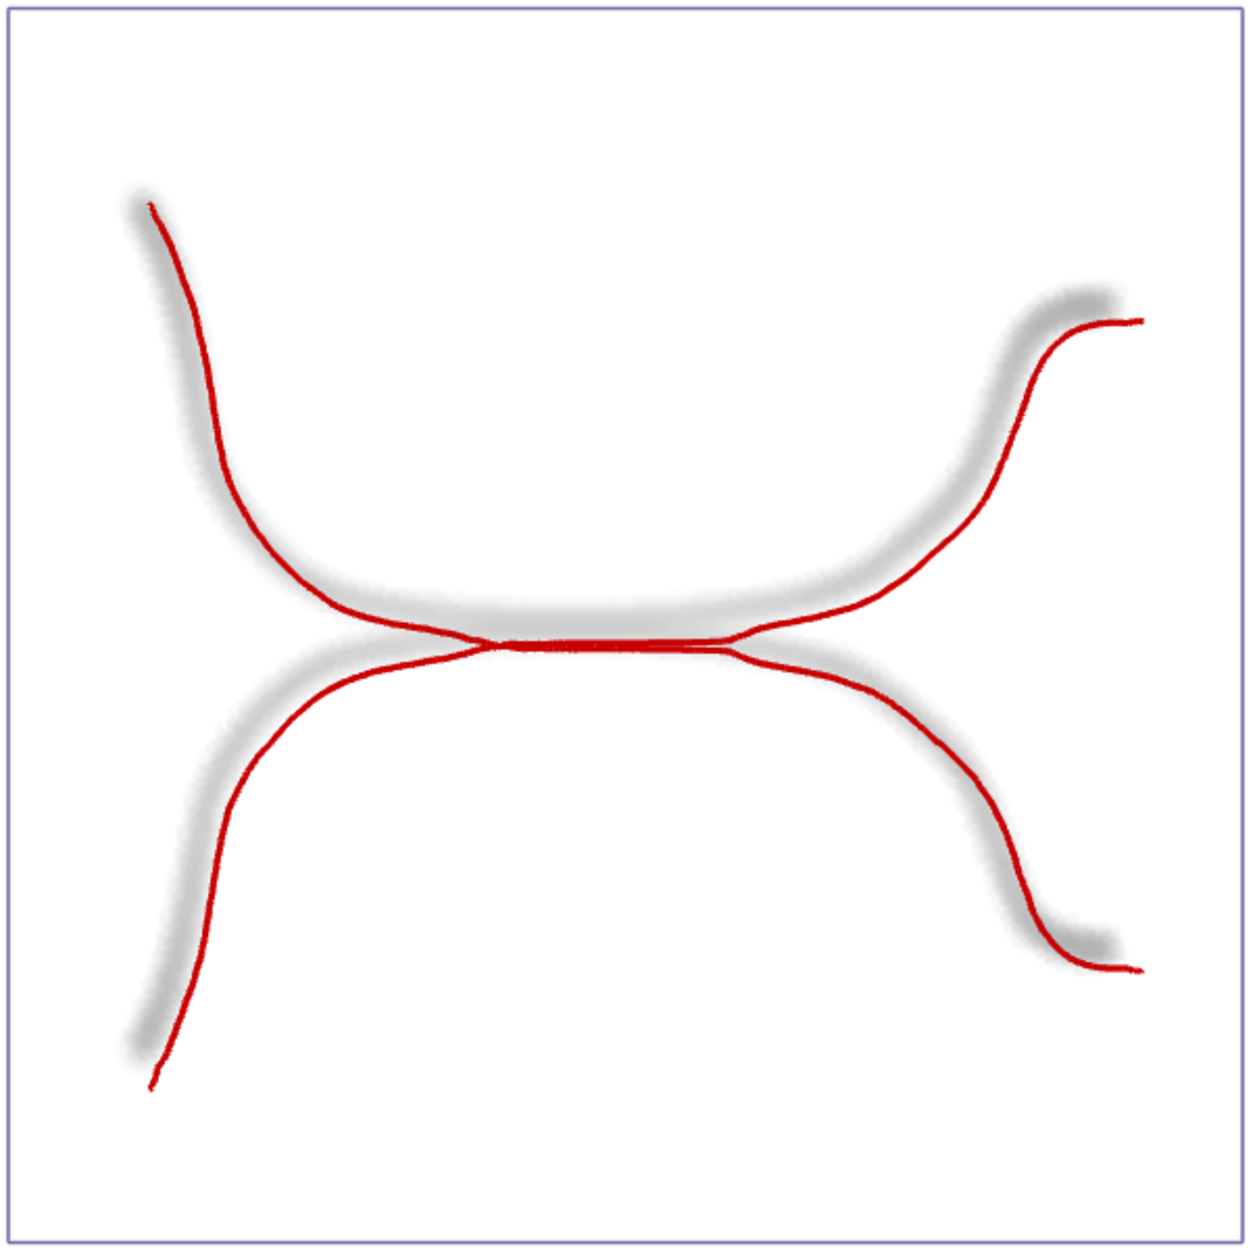
\includegraphics[align=c,width=0.2\columnwidth]{./fig/c2.compare/gps,i1} &
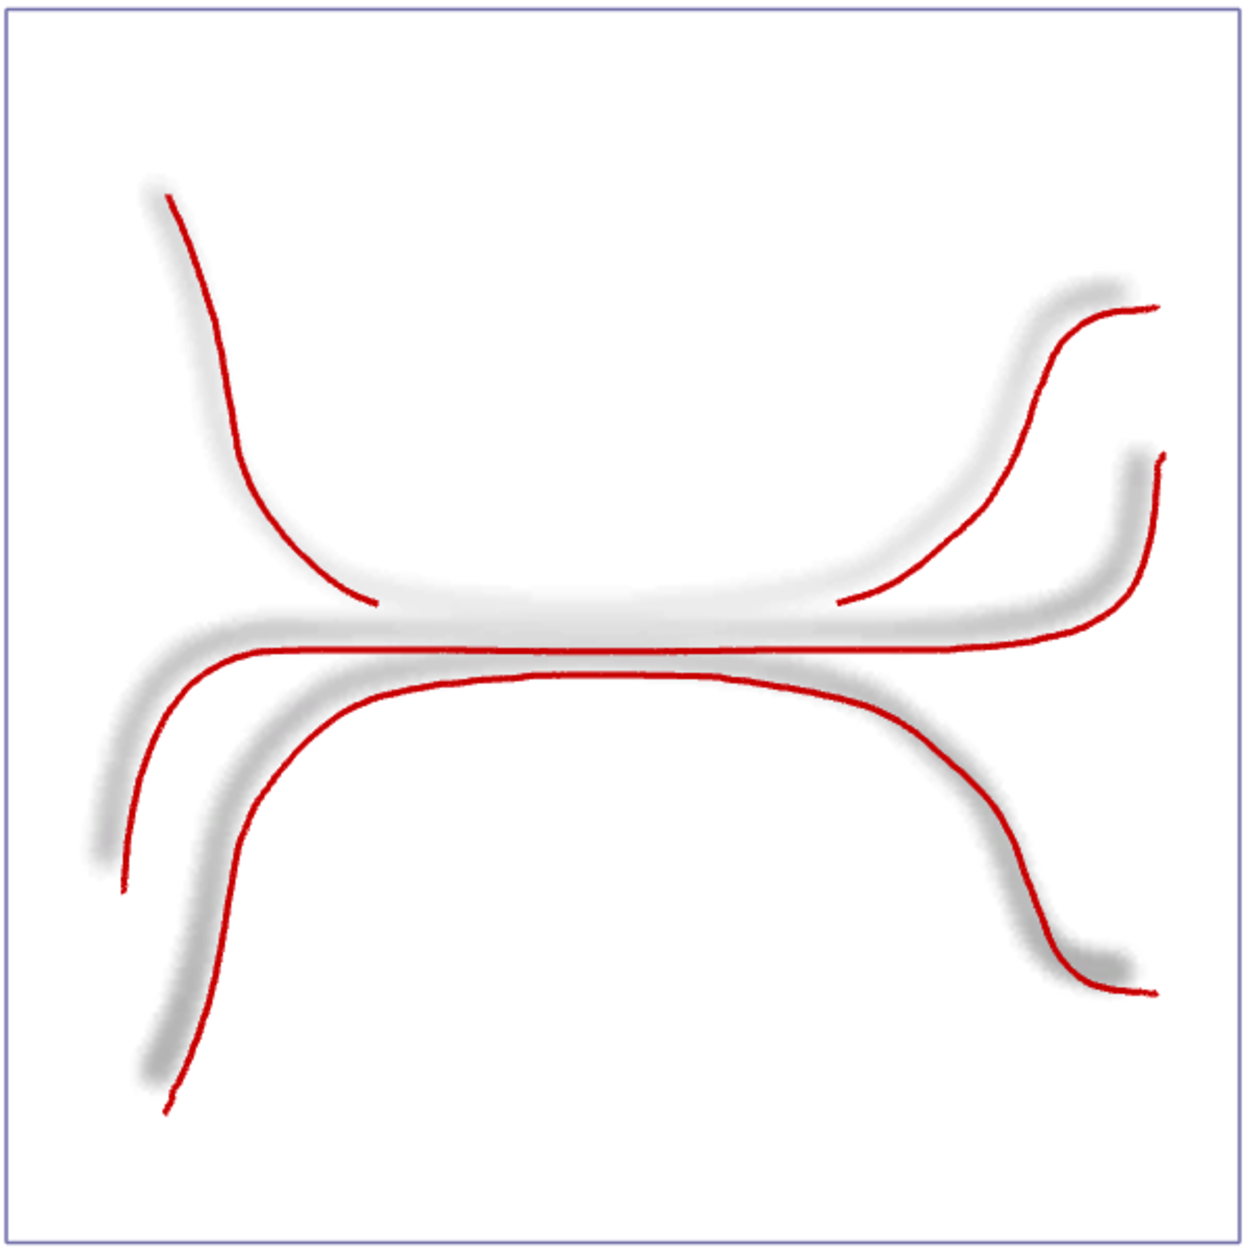
\includegraphics[align=c,width=0.2\columnwidth]{./fig/c2.compare/gps,i2} &
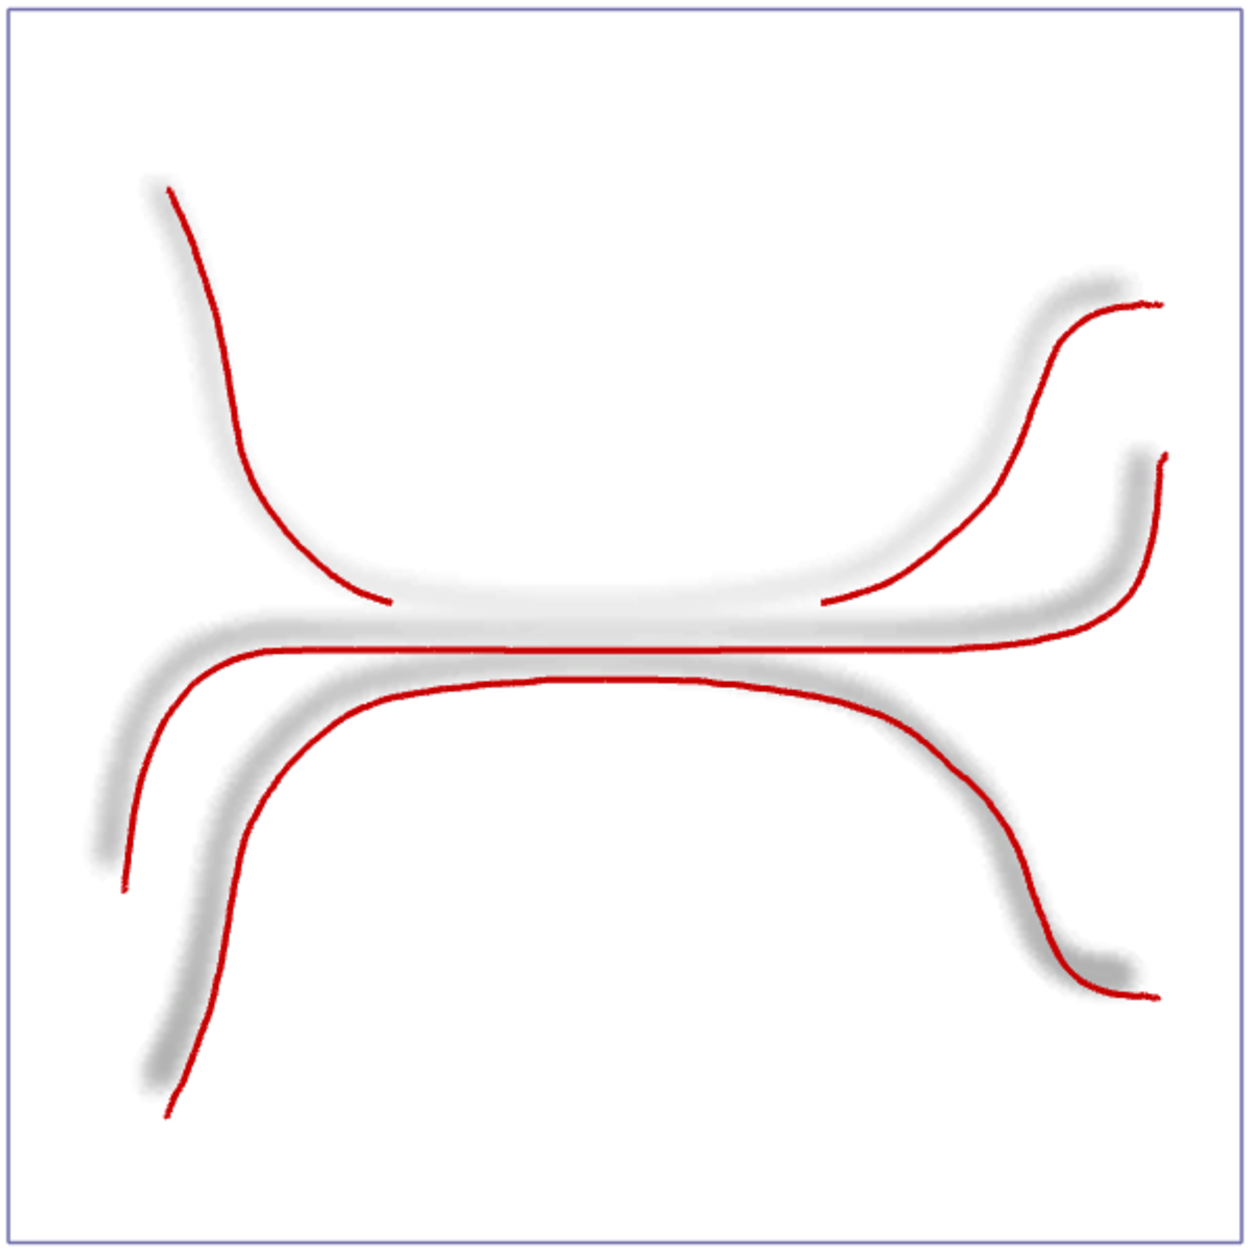
\includegraphics[align=c,width=0.2\columnwidth]{./fig/c2.compare/gps,i3} \\
APP2: &
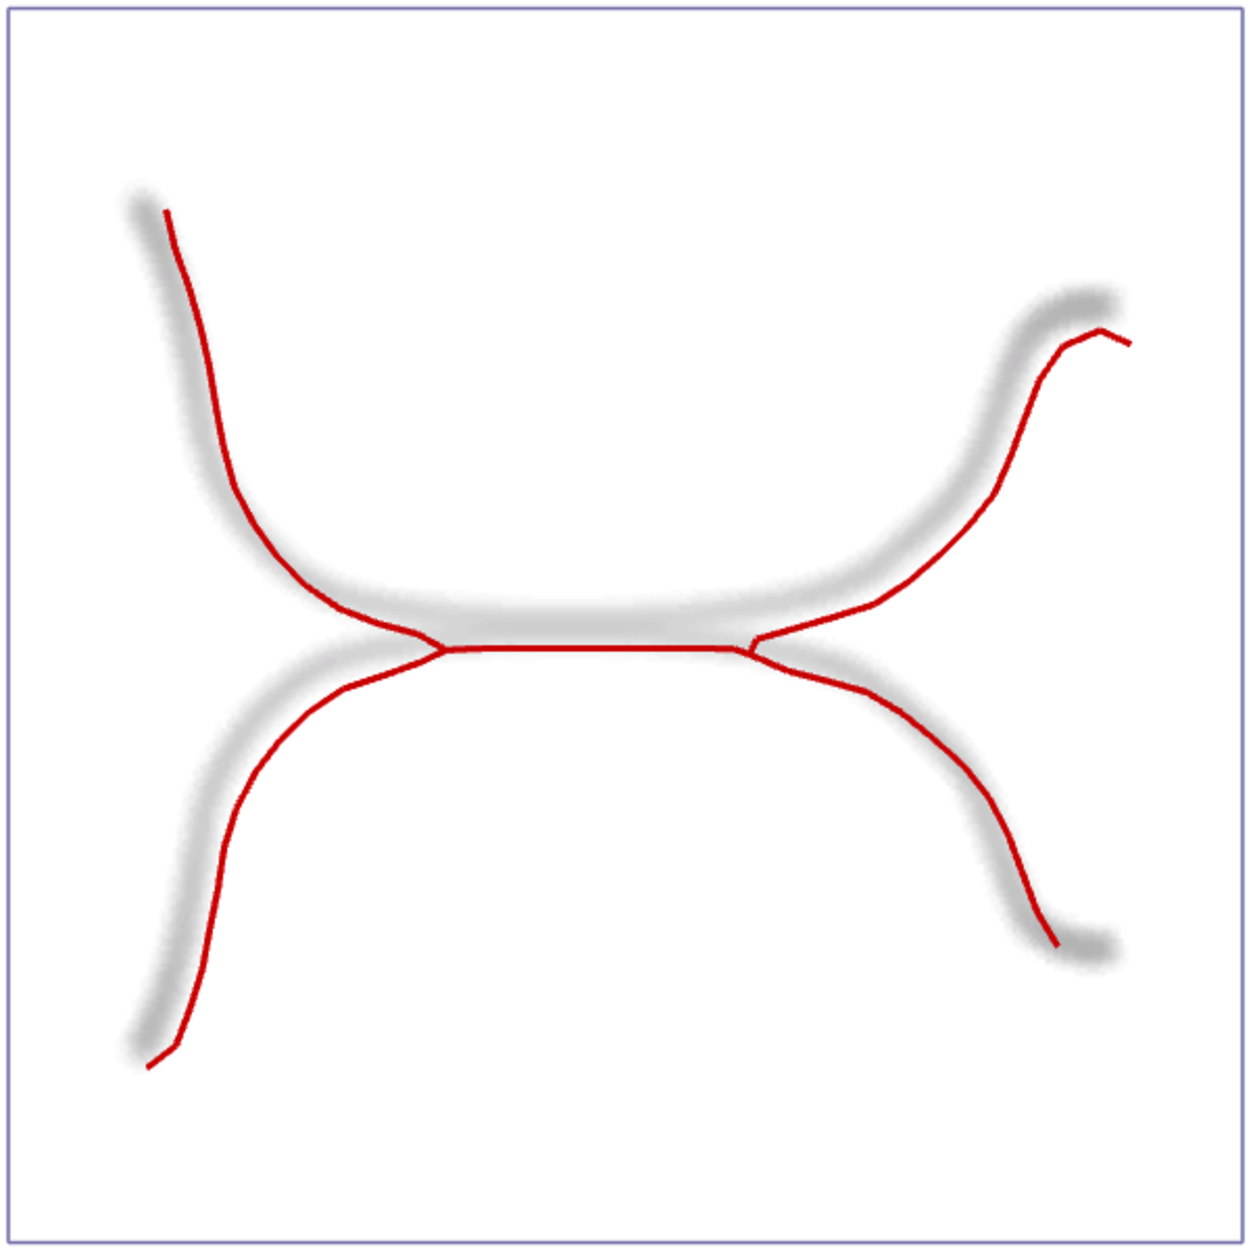
\includegraphics[align=c,width=0.2\columnwidth]{./fig/c2.compare/app2,i1} &
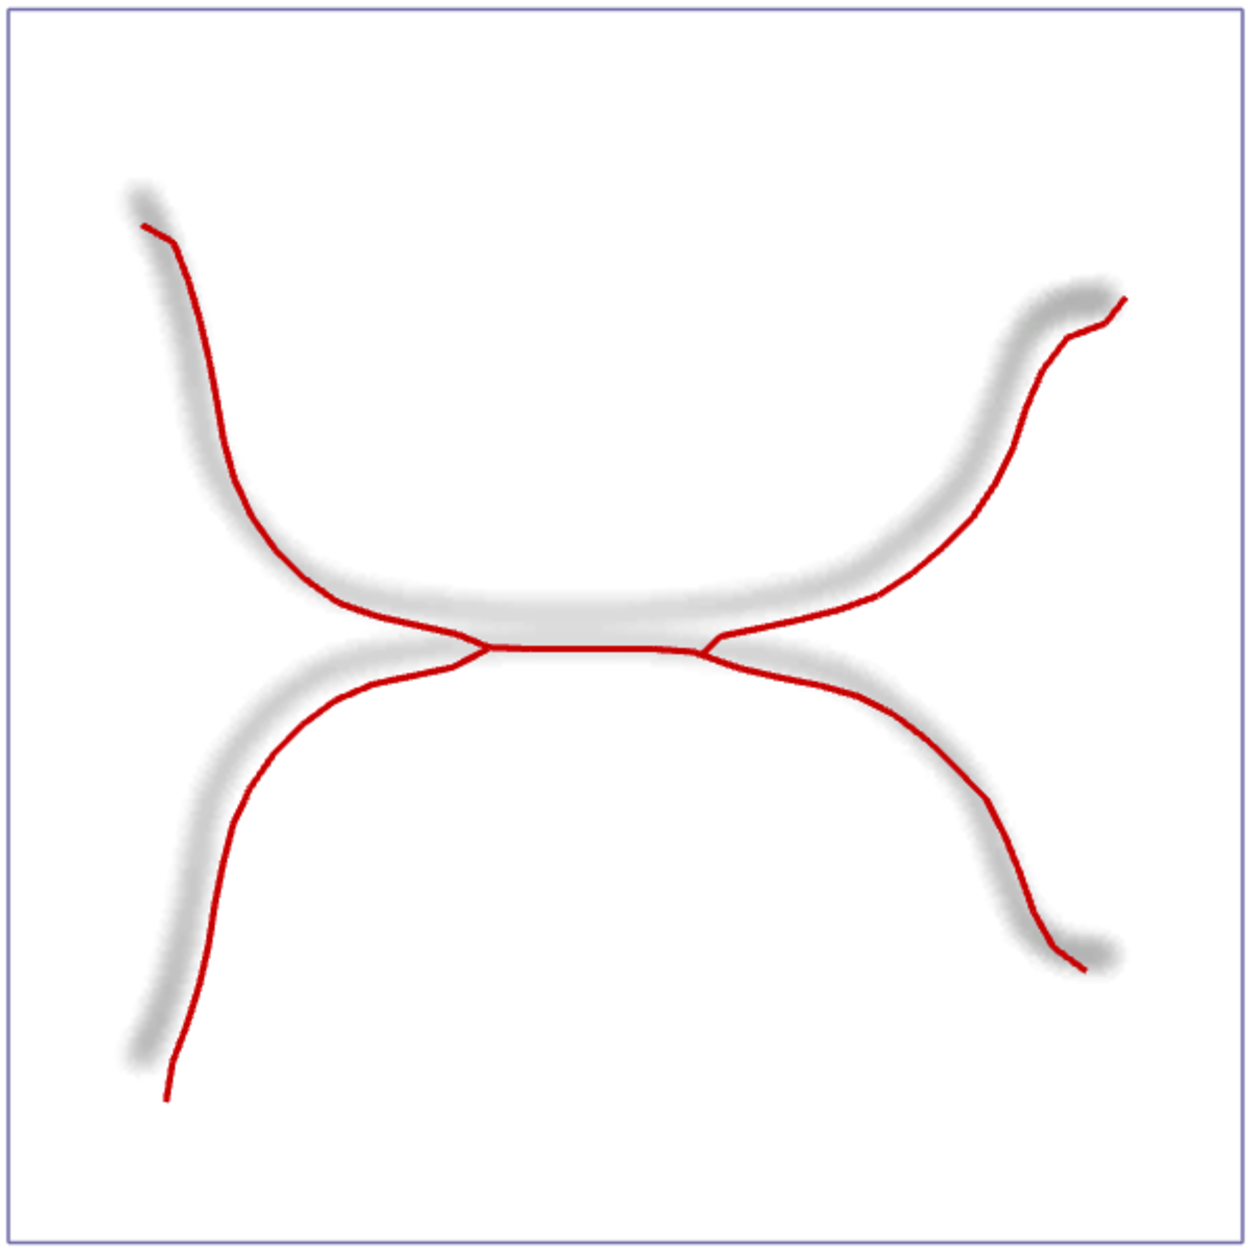
\includegraphics[align=c,width=0.2\columnwidth]{./fig/c2.compare/app2,i2} &
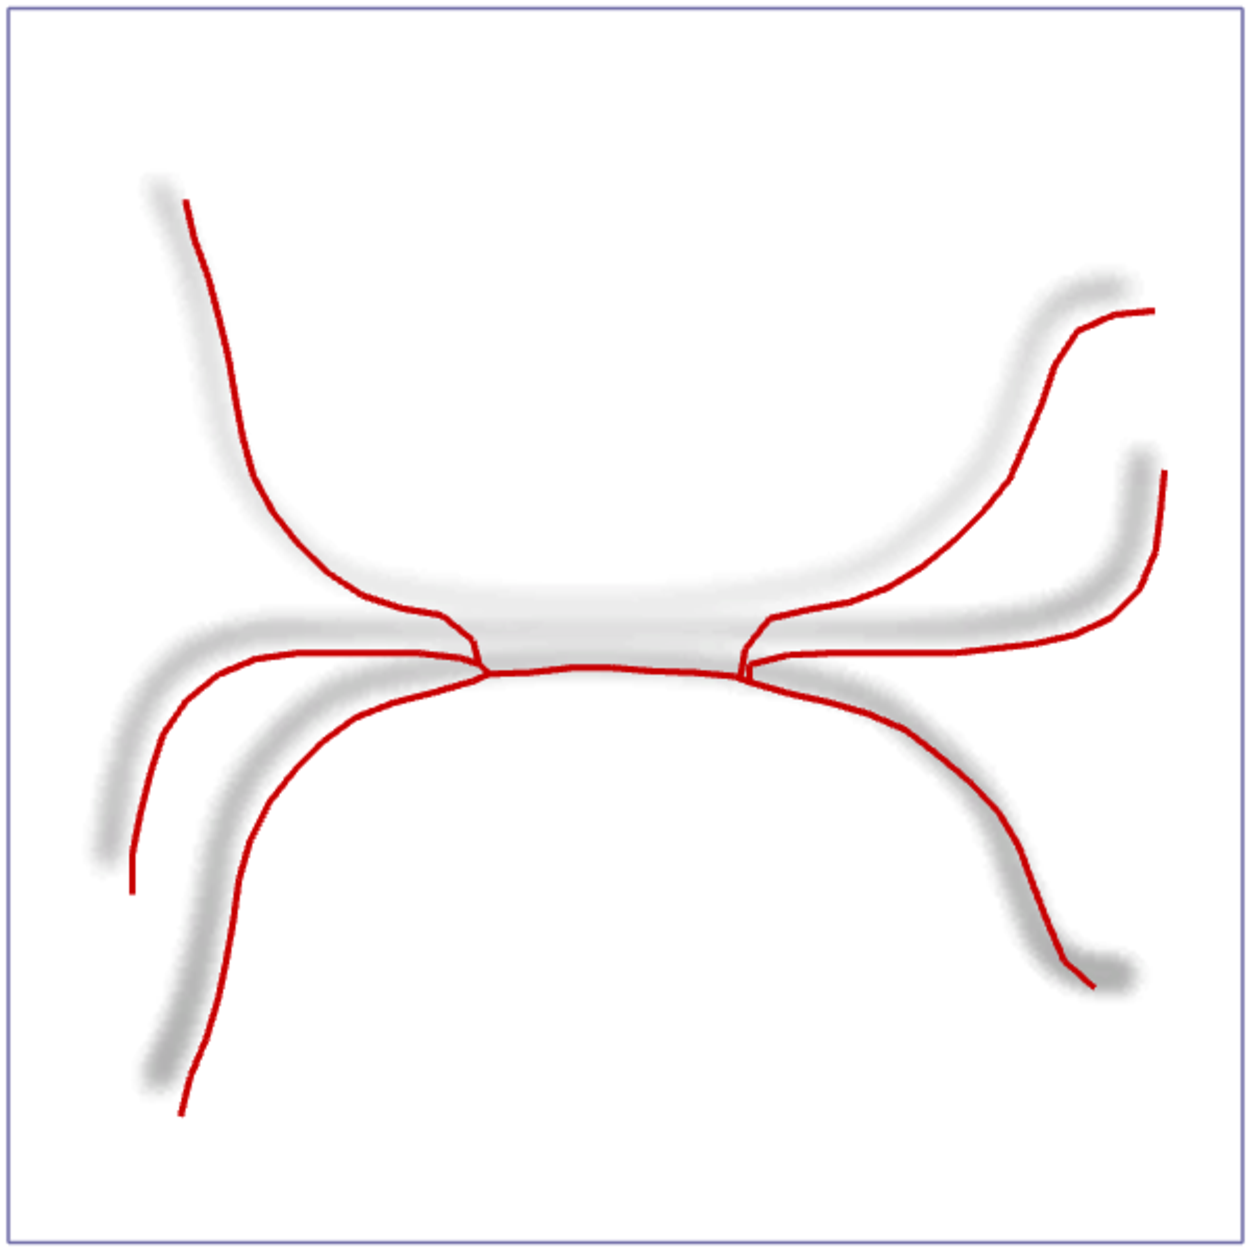
\includegraphics[align=c,width=0.2\columnwidth]{./fig/c2.compare/app2,i3} \\
MST: &
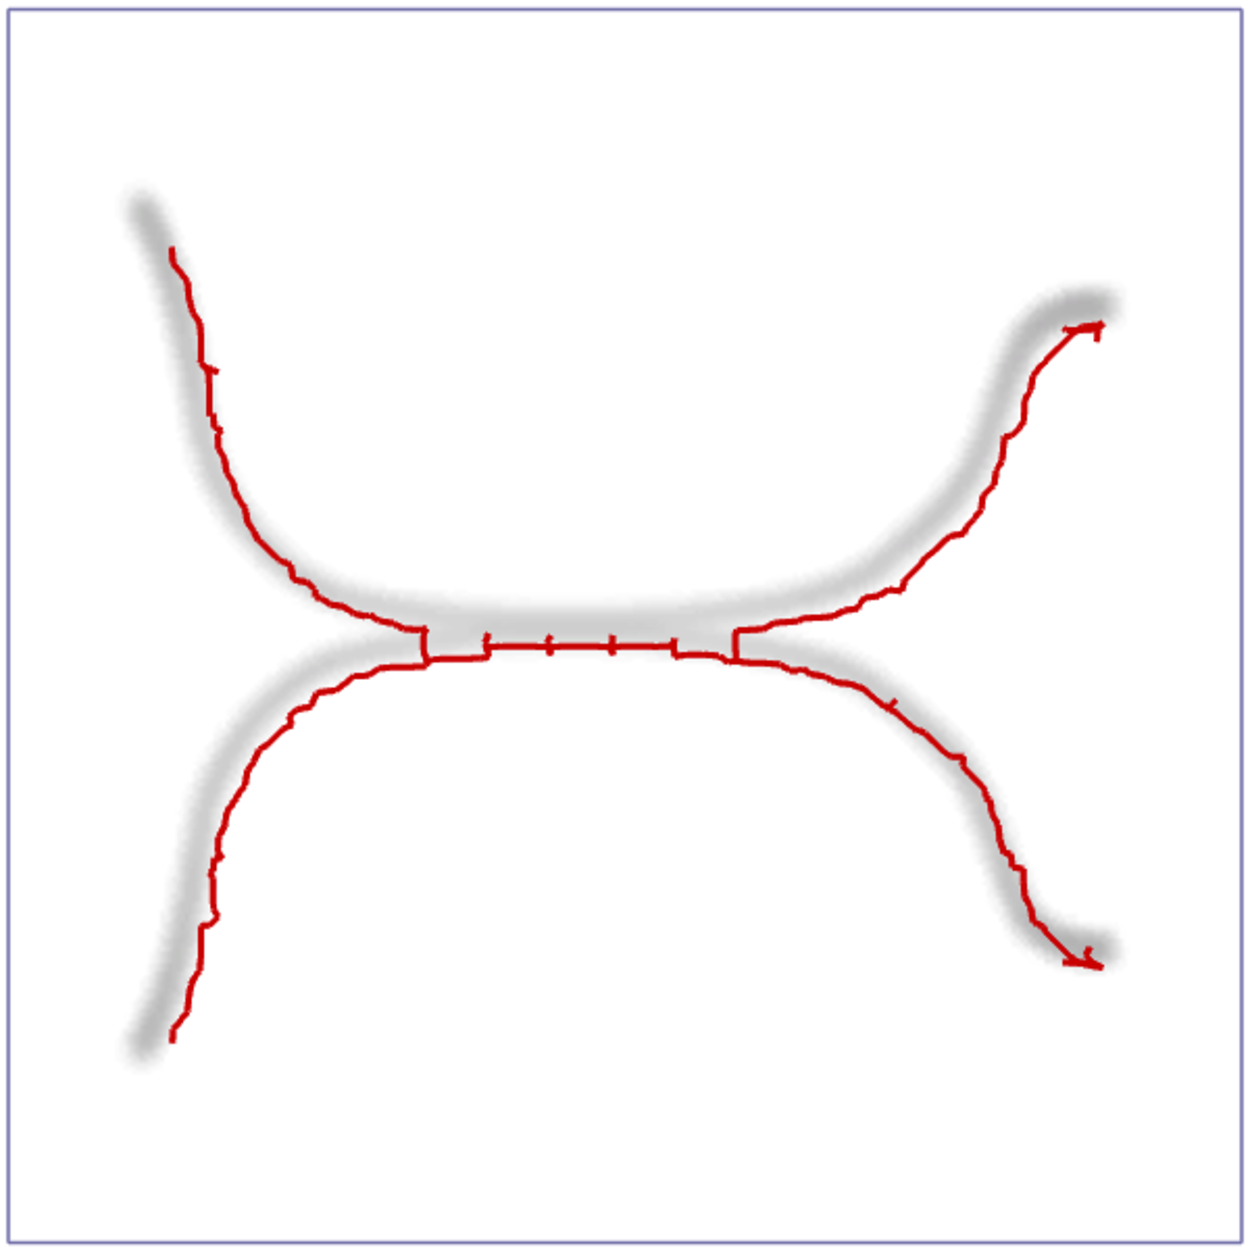
\includegraphics[align=c,width=0.2\columnwidth]{./fig/c2.compare/mst,i1} &
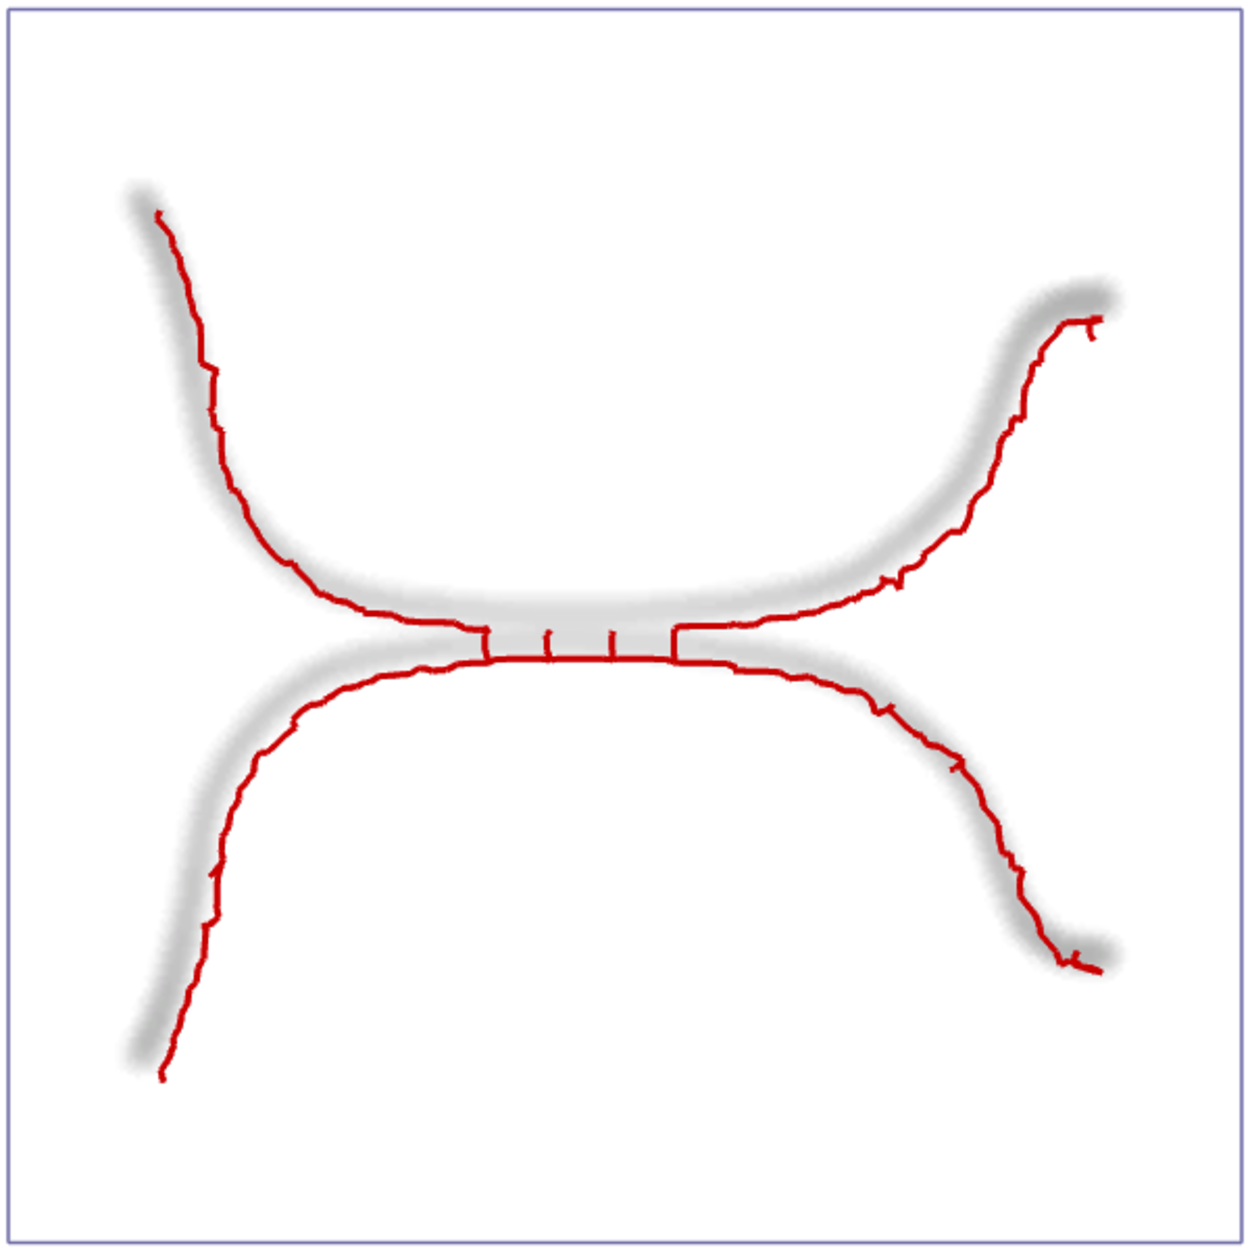
\includegraphics[align=c,width=0.2\columnwidth]{./fig/c2.compare/mst,i2} &
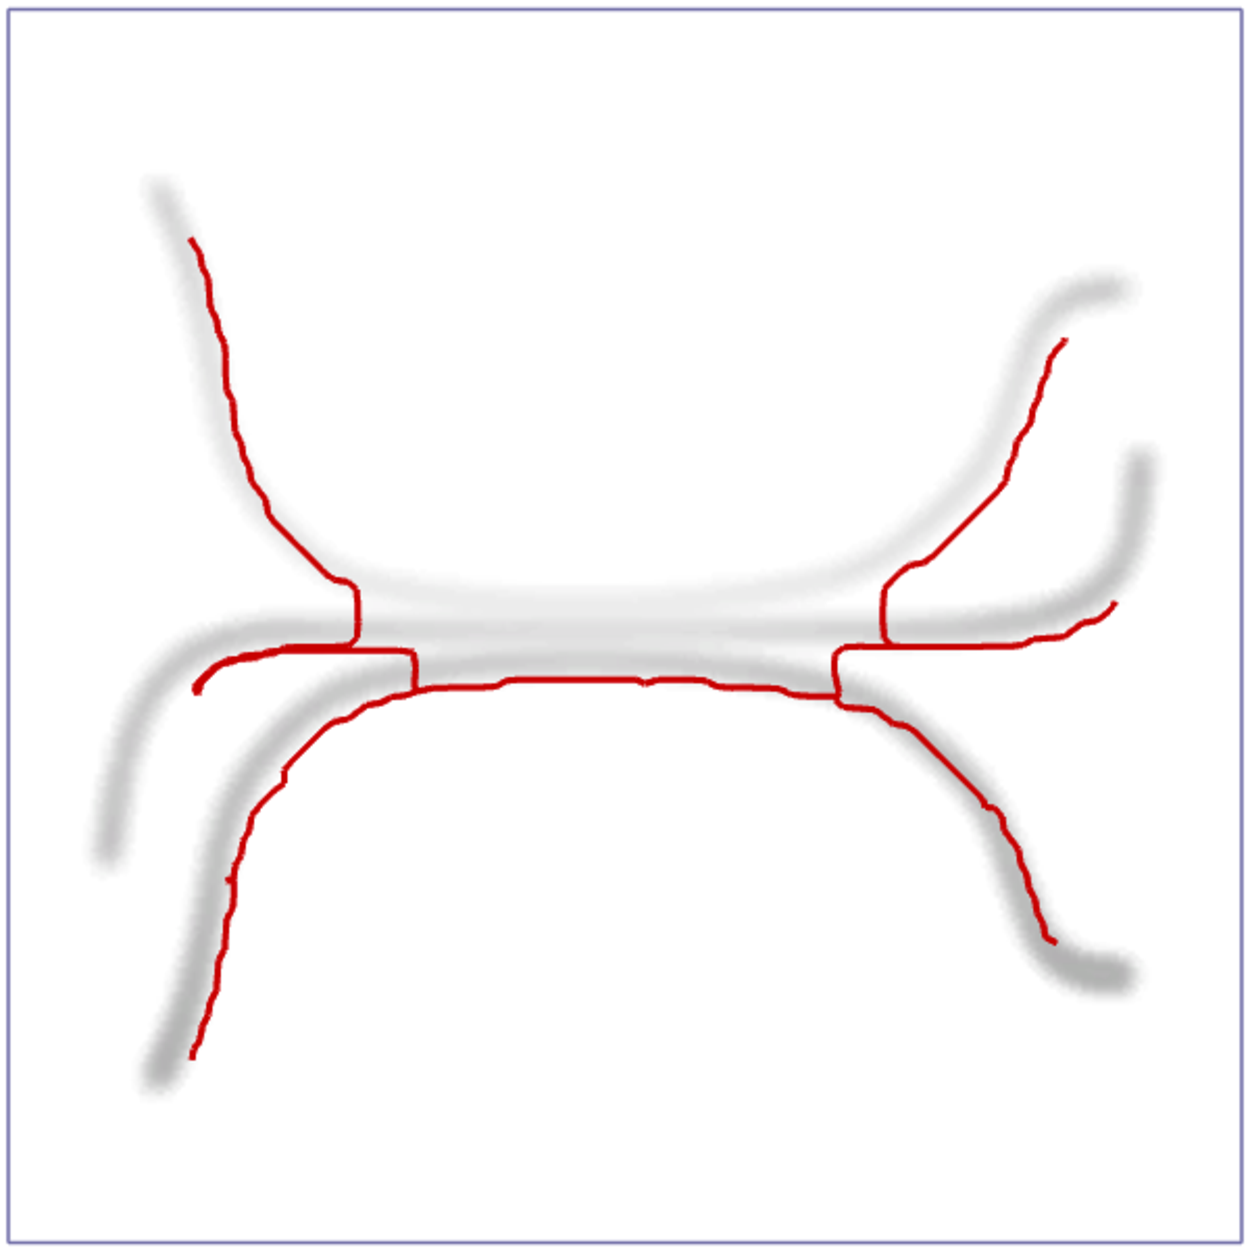
\includegraphics[align=c,width=0.2\columnwidth]{./fig/c2.compare/mst,i3} \\
\end{tabular}
\caption{Ability of the tested methods to separate two fibers of similar intensity and scale running closely in parallel. The examples show cases with gradually increasing distance between the fibers: overlap (left column), just separated (middle column), and clearly separated (right column). The tracing results of PHD, GPS, APP2, MST are overlaid (with slight offset) in red color.}
\label{fig:phd-advantage-2}
\end{figure}

% ************************************************************************
\clearpage
\begin{figure}[!t]
\centering
\begin{tabular}{c@{\hspace{0.02\columnwidth}}c@{\hspace{0.02\columnwidth}}c@{\hspace{0.02\columnwidth}}c}
%\multicolumn{4}{c}{\includegraphics[align=c,width=0.2\columnwidth]{./fig/test2d.compare/i}}\\
Case: &
\includegraphics[align=c,width=0.15\columnwidth]{./fig/c3.compare/i1_inv} &
\includegraphics[align=c,width=0.15\columnwidth]{./fig/c3.compare/i2_inv} &
\includegraphics[align=c,width=0.15\columnwidth]{./fig/c3.compare/i3_inv}\\
PHD: &
\includegraphics[align=c,width=0.2\columnwidth]{./fig/c3.compare/phd,i1,c0,s0} &
\includegraphics[align=c,width=0.2\columnwidth]{./fig/c3.compare/phd,i2,c0,s0} &
\includegraphics[align=c,width=0.2\columnwidth]{./fig/c3.compare/phd,i3,c0,s0} \\
GPS: &
\includegraphics[align=c,width=0.2\columnwidth]{./fig/c3.compare/gps,i1} &
\includegraphics[align=c,width=0.2\columnwidth]{./fig/c3.compare/gps,i2} &
\includegraphics[align=c,width=0.2\columnwidth]{./fig/c3.compare/gps,i3} \\
APP2: &
\includegraphics[align=c,width=0.2\columnwidth]{./fig/c3.compare/app2,i1} &
\includegraphics[align=c,width=0.2\columnwidth]{./fig/c3.compare/app2,i2} &
\includegraphics[align=c,width=0.2\columnwidth]{./fig/c3.compare/app2,i3} \\
MST: &
\includegraphics[align=c,width=0.2\columnwidth]{./fig/c3.compare/mst,i1} &
\includegraphics[align=c,width=0.2\columnwidth]{./fig/c3.compare/mst,i2} &
\includegraphics[align=c,width=0.2\columnwidth]{./fig/c3.compare/mst,i3} \\
\end{tabular}
\caption{Ability of the tested methods to separate three fibers with different intensity and scale running closely in parallel. The examples show cases with gradually increasing distance between the fibers: overlap (left column), just separated (middle column), and clearly separated (right column). The tracing results of PHD, GPS, APP2, MST are overlaid (with slight offset) in red color.}
\label{fig:phd-advantage-3}
\end{figure}

% ************************************************************************
\end{document}
% ************************************************************************